\documentclass[11pt]{article}

\usepackage[margin=1.6cm]{geometry}
\usepackage{amsmath}
\usepackage{amssymb}
\usepackage{enumitem}
\usepackage{titlesec}
\usepackage{xcolor}
\usepackage{fancyhdr}
\usepackage{tikz}
\usepackage{pgfplots}
\usepackage{multicol}
\usepackage{array}
\pgfplotsset{compat=1.18}

\titleformat{\section}{\large\bfseries\color{blue!50!black}}{\thesection}{0.6em}{}
\titlespacing{\section}{0pt}{1.0em}{0.4em}
\titleformat{\subsection}{\normalsize\bfseries}{\thesubsection}{0.6em}{}
\titlespacing{\subsection}{0pt}{0.7em}{0.3em}

\setlength{\headheight}{14pt}

\pagestyle{fancy}
\fancyhf{}
\fancyhead[L]{Statistics Revision}
\fancyfoot[C]{\thepage}
\renewcommand{\headrulewidth}{0.4pt}

\fancypagestyle{firstpage}{%
  \fancyhf{}
  \fancyhead[L]{Statistics Revision}
  \fancyhead[R]{Name: \makebox[4cm]{\hrulefill}}
  \fancyfoot[C]{\thepage}
  \renewcommand{\headrulewidth}{0.4pt}
}

\newcommand{\ans}{\hrulefill}
\newcommand{\anshere}{\par\vspace{0.8em}\noindent\ans\par\vspace{1.1em}}
\setlist[enumerate,1]{leftmargin=1.4em, itemsep=1.0em, topsep=0.4em}
\setlength{\columnsep}{1.0cm}
\setlength{\columnseprule}{0.4pt}
\raggedcolumns

% axis box suited to all-positive scatter data: xmin xmax ymin ymax xtick ytick xlabel ylabel
\newcommand{\scatteraxis}[8]{%
  \begin{axis}[
    width=8.0cm, height=5.6cm,
    xmin=#1, xmax=#2, ymin=#3, ymax=#4,
    xtick distance=#5, ytick distance=#6,
    grid=both, grid style={line width=.1pt, draw=gray!35},
    axis lines=left,
    xlabel={#7}, ylabel={#8},
    tick label style={font=\tiny},
    label style={font=\small},
  ]
}

\newcommand{\mistake}[1]{%
  \begin{center}
  \fcolorbox{red!55!black}{red!6}{\parbox{0.96\linewidth}{\small\textbf{Common mistake:} #1}}
  \end{center}
}

\begin{document}
\thispagestyle{firstpage}

\begin{center}
  {\Large\bfseries Statistics Revision}\\[2pt]
  {\normalsize Scatter Plots, Spread and Centre}
\end{center}
\vspace{0.3em}

\section{Scatter Plots and Lines of Best Fit}

\noindent A \textbf{line of best fit} is a straight line drawn through scatter data that follows
the overall trend, with roughly equal numbers of points above and below it. To \textbf{estimate} a
value, you must draw this line first and then read your estimate \emph{from the line} --- not from
whichever data point happens to be nearest.

\mistake{Reading an estimate straight off the nearest data point, without drawing a line of best
fit first. This is especially risky when there is a gap in the data near the value you need ---
without a line, there is nothing reliable to read from.}

\subsection*{Worked example}
\noindent The scatter graph shows hours studied per week against test score for 15 students.
Estimate the test score for a student who studied for 6 hours.

\begin{center}
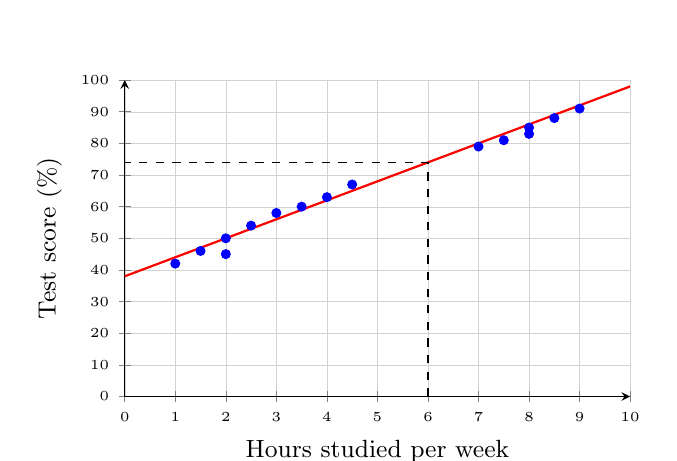
\begin{tikzpicture}
\scatteraxis{0}{10}{0}{100}{1}{10}{Hours studied per week}{Test score (\%)}
\addplot[only marks, mark=*, mark size=1.6pt, blue] coordinates {
  (1,42) (1.5,46) (2,50) (2,45) (2.5,54) (3,58) (3.5,60) (4,63) (4.5,67)
  (7,79) (7.5,81) (8,85) (8,83) (8.5,88) (9,91)
};
\addplot[domain=0:10, samples=2, thick, red] {6*x+38};
\draw[dashed] (axis cs:6,0) -- (axis cs:6,74) -- (axis cs:0,74);
\end{axis}
\end{tikzpicture}
\end{center}

\noindent\textbf{Step 1:} Draw a line of best fit through the data (shown in red). \\
\noindent\textbf{Step 2:} Find $6$ on the \emph{hours studied} axis, go straight up to the line,
then straight across to the \emph{test score} axis (dashed lines). \\
\noindent\textbf{Step 3:} Read off the estimate: a student who studied for $6$ hours is estimated
to score about $\mathbf{74\%}$. \quad (Notice there is no data point at $6$ hours --- the line is
the only reliable way to estimate this.)

\vspace{0.6em}
\noindent\textbf{Try it yourself:} Using the \emph{same} line of best fit above, estimate the test
score for a student who studied for $2.5$ hours per week.
\anshere

\newpage

\subsection*{Practice}
\noindent For each scatter graph: (a) draw a line of best fit by eye, (b) use your line to make
the estimate asked for, and (c) answer the follow-up questions.

\renewcommand{\anshere}{\par\vspace{0.2em}\noindent\ans\par\vspace{0.2em}}
\setlist[enumerate,1]{leftmargin=1.4em, itemsep=0.3em, topsep=0.2em}

\vspace{0.3em}
\noindent\textbf{1. Hours of sleep vs reaction time}

\begin{center}
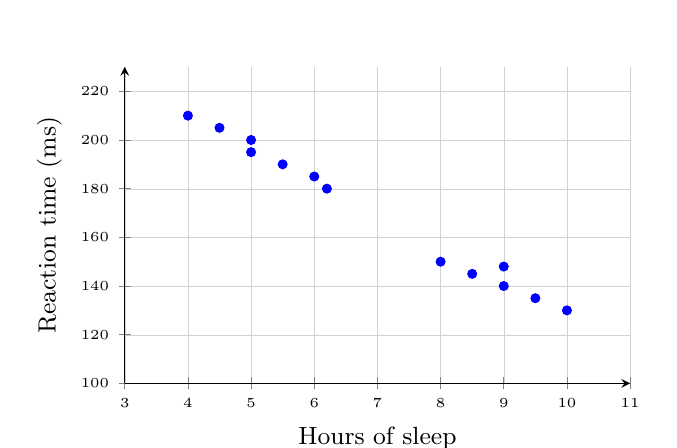
\begin{tikzpicture}
\scatteraxis{3}{11}{100}{230}{1}{20}{Hours of sleep}{Reaction time (ms)}
\addplot[only marks, mark=*, mark size=1.6pt, blue] coordinates {
  (4,210) (4.5,205) (5,195) (5,200) (5.5,190) (6,185) (6.2,180)
  (8,150) (8.5,145) (9,140) (9,148) (9.5,135) (10,130)
};
\end{axis}
\end{tikzpicture}
\end{center}

\begin{enumerate}[label=(\alph*)]
  \item Use your line of best fit to estimate the reaction time for someone who sleeps for
    $7$ hours.
  \anshere
  \item Describe the correlation shown in the scatter graph (direction and strength).
  \anshere
  \item Why is a line of best fit especially necessary for part (a), rather than just reading
    off a nearby point?
  \anshere
\end{enumerate}

\vspace{0.4em}
\noindent\textbf{2. Weekly training distance vs race time}

\begin{center}
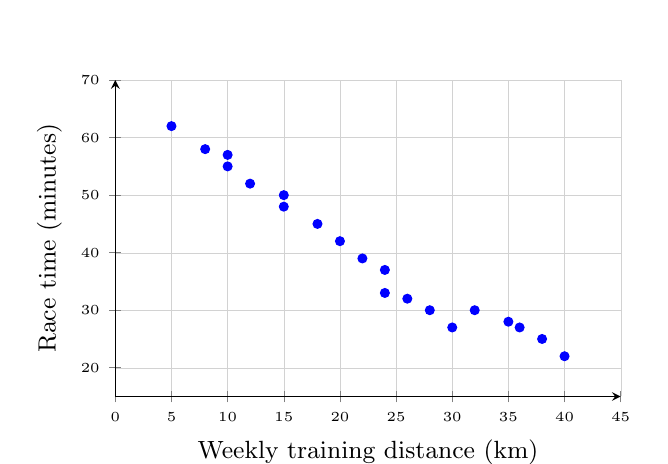
\begin{tikzpicture}
\scatteraxis{0}{45}{15}{70}{5}{10}{Weekly training distance (km)}{Race time (minutes)}
\addplot[only marks, mark=*, mark size=1.6pt, blue] coordinates {
  (5,62) (8,58) (10,55) (10,57) (12,52) (15,48) (15,50) (18,45)
  (20,42) (22,39) (24,33) (24,37) (26,32) (28,30) (30,27)
  (32,30) (35,28) (36,27) (38,25) (40,22)
};
\end{axis}
\end{tikzpicture}
\end{center}

\begin{enumerate}[label=(\alph*)]
  \item Use your line of best fit to estimate the race time for a runner who trains
    $25$\,km per week.
  \anshere
  \item There are data points close to $25$\,km. Explain why you should still read your estimate
    from the line, rather than just from one of those nearby points.
  \anshere
  \item Use your line to estimate the race time for a runner who trains $0$\,km per week.
    Explain why this particular estimate might \emph{not} be reliable, even though you used a
    line of best fit.
  \anshere
\end{enumerate}

\newpage

\renewcommand{\anshere}{\par\vspace{0.8em}\noindent\ans\par\vspace{1.1em}}
\setlist[enumerate,1]{leftmargin=1.4em, itemsep=1.0em, topsep=0.4em}

\section{Comparing Spread (Consistency)}

\noindent Imagine two archers each shoot $8$ arrows at a target.

\begin{center}
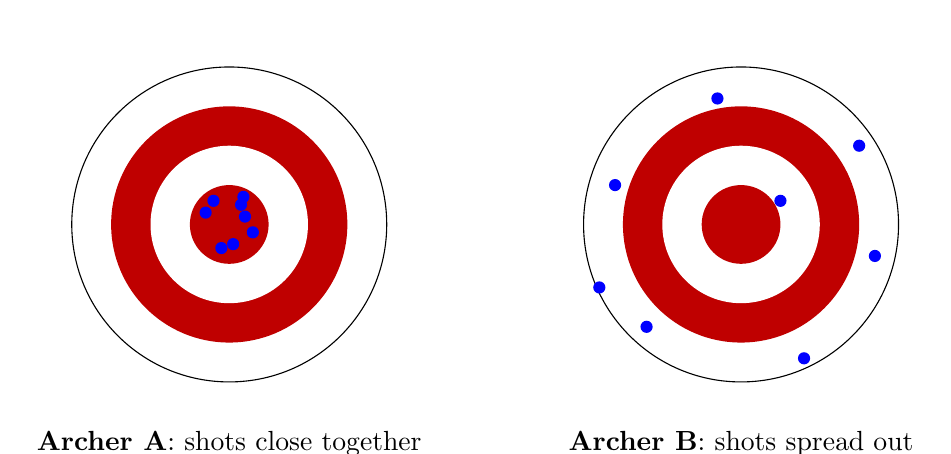
\begin{tikzpicture}
\begin{scope}
  \foreach \r/\col in {2/white, 1.5/red!75!black, 1/white, 0.5/red!75!black} {\fill[\col] (0,0) circle (\r);}
  \draw (0,0) circle (2);
  \foreach \p in {(0.15,0.25),(-0.2,0.3),(0.3,-0.1),(-0.1,-0.3),(0.2,0.1),(-0.3,0.15),(0.05,-0.25),(0.18,0.35)}
    \fill[blue] \p circle (2.2pt);
  \node[below] at (0,-2.5) {\textbf{Archer A}: shots close together};
\end{scope}
\begin{scope}[xshift=6.5cm]
  \foreach \r/\col in {2/white, 1.5/red!75!black, 1/white, 0.5/red!75!black} {\fill[\col] (0,0) circle (\r);}
  \draw (0,0) circle (2);
  \foreach \p in {(1.5,1.0),(-1.6,0.5),(0.8,-1.7),(-1.2,-1.3),(1.7,-0.4),(-0.3,1.6),(0.5,0.3),(-1.8,-0.8)}
    \fill[blue] \p circle (2.2pt);
  \node[below] at (0,-2.5) {\textbf{Archer B}: shots spread out};
\end{scope}
\end{tikzpicture}
\end{center}

\noindent Archer A's arrows landed close together --- \textbf{consistent} shooting, even though not
every shot hit the bullseye. Archer B's arrows landed all over the target --- \textbf{inconsistent}
shooting: the more spread out the points are, the less consistent they are. Data works the same way.

\vspace{0.4em}
\noindent \textbf{Spread} tells us how varied or consistent a data set is. The \textbf{range}
(largest $-$ smallest) and the \textbf{IQR} (interquartile range) both measure spread.
\begin{center}
\textbf{Smaller spread} $\Rightarrow$ values are closer together $\Rightarrow$ \emph{more
consistent}.\\
\textbf{Larger spread} $\Rightarrow$ values are more varied $\Rightarrow$ \emph{less consistent}.
\end{center}

\mistake{Writing that the group with the \emph{larger} range or IQR is ``more consistent.'' It is
the opposite: a larger range means the data values are more spread out and \emph{less} alike, so
that group is \emph{less} consistent.}

\subsection*{Worked example}
\noindent Daily exercise times (minutes) for two groups over 8 days:
\[
  \text{Group A: } 25,\,26,\,27,\,28,\,29,\,30,\,31,\,32 \qquad
  \text{Group B: } 10,\,15,\,20,\,25,\,40,\,45,\,50,\,55
\]
Which group has more consistent exercise times?

\vspace{0.3em}
\noindent Range of Group A $= 32-25=7$ minutes. \quad Range of Group B $=55-10=45$ minutes.

\vspace{0.3em}
\noindent\textbf{Answer:} Group A is more consistent, because it has the \emph{smaller} range
($7$ minutes, compared to Group B's $45$ minutes). This means Group A's exercise times are all
similar to each other, while Group B's times vary a lot from day to day.

\vspace{0.6em}
\subsection*{Practice}
\noindent Judges' scores (out of 10) for two gymnasts over 10 routines:
\[
  \text{Gymnast X: } 7.2,7.3,7.4,7.4,7.5,7.5,7.6,7.6,7.7,7.8 \qquad
  \text{Gymnast Y: } 5.0,5.5,6.2,6.8,7.0,8.5,8.8,9.0,9.2,9.5
\]

\begin{enumerate}[label=(\alph*)]
  \item Calculate the range for each gymnast.
  \anshere
  \item Which gymnast scored more consistently? Write a full answer, using your ranges, that
    explains \emph{why} a smaller range means more consistent scoring.
  \anshere
\end{enumerate}

\newpage

\section{Comparing Centre (Typical Value)}

\noindent \textbf{Measures of centre} (mean, median) tell us about a \emph{typical} value in a data
set --- this is a completely different question from spread/consistency.
\begin{center}
\textbf{Spread} $\longrightarrow$ how consistent the data is. \qquad
\textbf{Centre} $\longrightarrow$ what a typical value is.
\end{center}
\noindent Be careful: whether a \emph{higher} or \emph{lower} value is ``better'' depends on the
context. A higher mean test score is better, but a lower mean race time is better.

\subsection*{Worked example 1 (higher is better)}
\noindent Mean test scores: Class 1 $=74\%$, Class 2 $=61.5\%$.
\noindent\textbf{Answer:} Class 1 typically scored higher, because its mean ($74\%$) is greater
than Class 2's mean ($61.5\%$).

\vspace{0.4em}
\subsection*{Worked example 2 (lower is better)}
\noindent Mean race times: Swimmer P $=31.08$\,s, Swimmer Q $=29.53$\,s.
\noindent\textbf{Answer:} Swimmer Q was typically faster, because a \emph{lower} mean time means
less time taken to finish the race --- even though $29.53$ is the smaller number, it is the better
result here.

\vspace{0.6em}
\subsection*{Mixed practice}
\noindent Scores out of 30 for two quiz teams over 8 rounds:
\[
  \text{Team Alpha: } 15,16,16,17,17,18,18,19 \qquad
  \text{Team Beta: } 5,8,10,12,22,25,28,30
\]

\begin{enumerate}[label=(\alph*)]
  \item Calculate the mean score for each team.
  \anshere
  \item Calculate the range for each team.
  \anshere
  \item Which team scored higher, on average? Justify your answer using your means.
  \anshere
  \item Which team was more consistent? Justify your answer using your ranges.
  \anshere
  \item Explain why your answers to (c) and (d) are both correct, even though they compare the
    teams in different ways.
  \anshere
\end{enumerate}

\end{document}
